\documentclass{article}
\usepackage[utf8]{inputenc}

\title{Laboratorio 1}
\author{Nicola Agostini, Roberto Cedolin, Lisa Parma}
\date{March 2019}

\usepackage{amsmath}
\usepackage{natbib}
\usepackage{graphicx}
\usepackage{placeins}
\usepackage{mathtools, nccmath}
\usepackage{hyperref}
\usepackage{biblatex}
\DeclarePairedDelimiter{\nint}\lfloor\rceil

\begin{document}

\maketitle

\section*{Introduzione}

In questo laboratorio si vuole analizzare la connettività di grafi diversi tra loro. In particolare viene utilizzato l'algoritmo UPA ed ER per la creazione di grafi in modo automatico e la lettura di un file di testo per la creazione di un grafo rappresentante una rete di calcolatori reale.


\section*{Domanda 1}
\begin{center}
\begin{figure}[h]
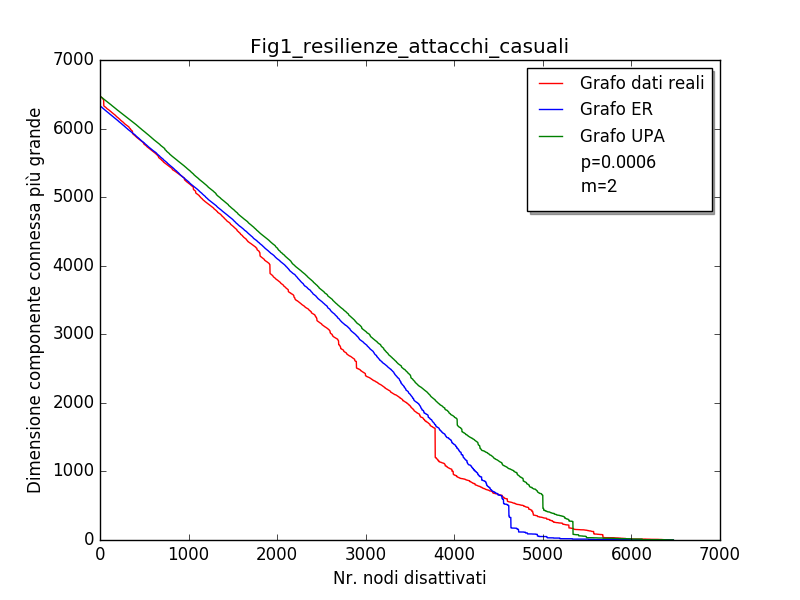
\includegraphics[scale=0.7, \textwidth, left]{Fig1_resilienze_attacchi_casuali.png}
\caption{Grafico domanda 1}
\label{fig:graph1}
\end{figure}
\end{center}

All'interno di \ref{fig:graph1} è rappresentato l'andamento della resilienza dei tre grafi (UPA, ER e dati reali) dopo la disattivazione di un numero crescente di nodi scelti casualmente. Come si può notare, il grafo che rappresenta i dati reali, a parità di nodi eliminati mostra generalmente una resilienza minore rispetto ai grafi generati con gli algoritmi ER ed UPA.\newline Il valore di p utilizzato per la creazione del grafo attraverso l'algoritmo ER è pari a 
\[
    \frac{12572}{\binom{6474}{2}}=0.000600
\]
questo perchè per avere un numero di archi pari a 12572 è necessario scegliere un arco ogni 6000 dal grafo completo. Quindi la probabilità di scegliere un arco è appunto 0.0006.
Il valore di m scelto è pari al grado medio dei vertici del grafo reale diviso per due. Il parametro m viene calcolato con 
\[
  \nint*{\frac{6474}{12572}}=2
\]
che è il grado medio dei nodi del grafo diviso 2.

\FloatBarrier

\section*{Domanda 2}
\begin{figure}[h]
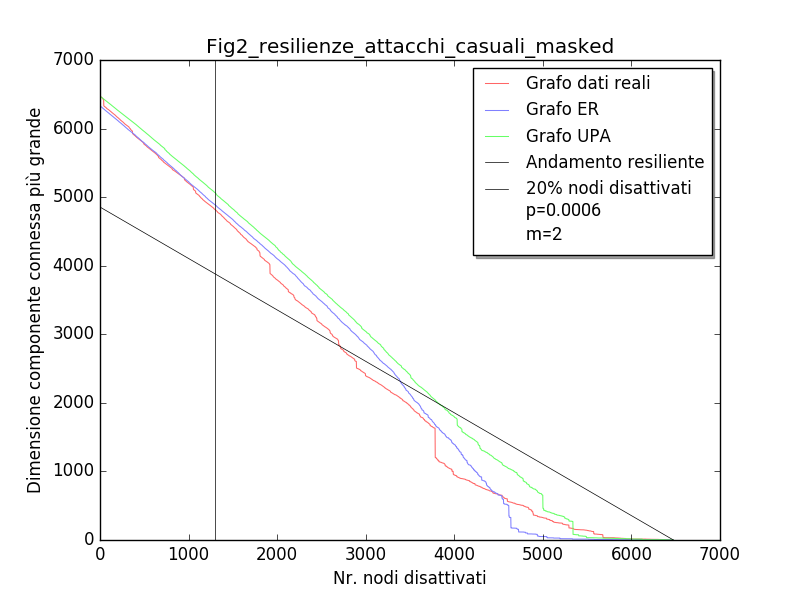
\includegraphics[scale=0.7, \textwidth, left]{Fig2_resilienze_attacchi_casuali_masked.png}
\caption{Grafico domanda 2}
\label{fig:graph2}
\end{figure}
Nel grafo \ref{fig:graph2} è sempre presente l'andamento delle tre curve dei grafi dopo la rimozione di nodi, sono presenti anche due rette, una verticale in posizione dei 20\% dei nodi disattivati, l'altra che indica quando la dimensione della componente connessa più grande è superiore al 75\% del numero dei nodi ancora attivi.
Perciò un grafo è resiliente quando in corrispondenza della sua intersezione con la retta verticale (20\% dei nodi disattivati) il punto di intersezione è al di sopra della retta grigia inclinata che indica appunto quando un grafo è resiliente.
In questo caso tutti e tre i grafi sono resilienti.
\FloatBarrier
\section*{Domanda 3}
\begin{center}
\begin{figure}[h]
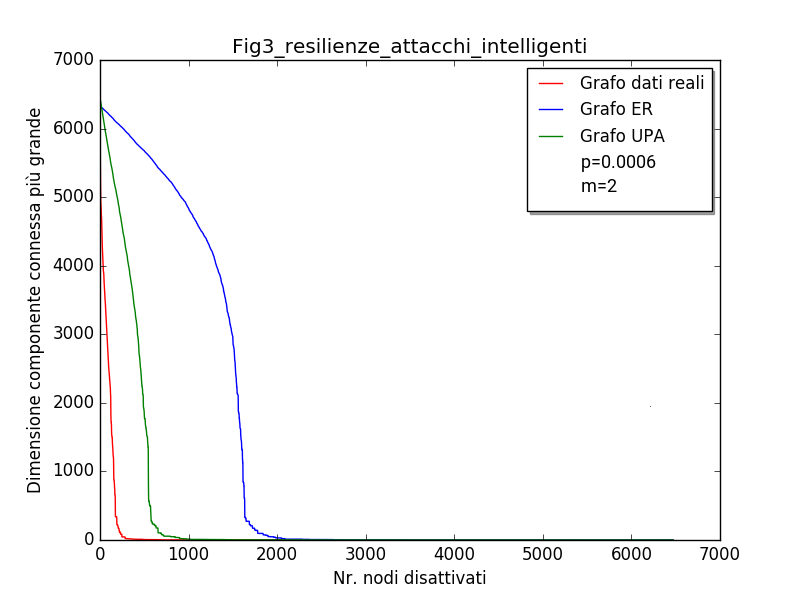
\includegraphics[scale=0.7, \textwidth, left]{Fig3_resilienze_attacchi_intelligenti.png}
\caption{Grafico domanda 3}
\label{fig:graph3}
\end{figure}
\end{center}
Nel grafico in figura \ref{fig:graph3} vi è l'andamento dei tre grafi dopo che subiscono un attacco che disattiva in nodi scegliendo quelli con grado maggiore.
Si nota che a parità di nodi disattivati il grafo ER mantiene una componente connessa maggiore rispetto al grafo UPA e quello dei dati reali.
Questo è dovuto al fatto che l'algoritmo ER collega casualmente i nodi in modo tale da avere una rete più resistente a questo tipo di attacchi.

\FloatBarrier

\section*{Domanda 4}
\begin{center}
\begin{figure}[h]
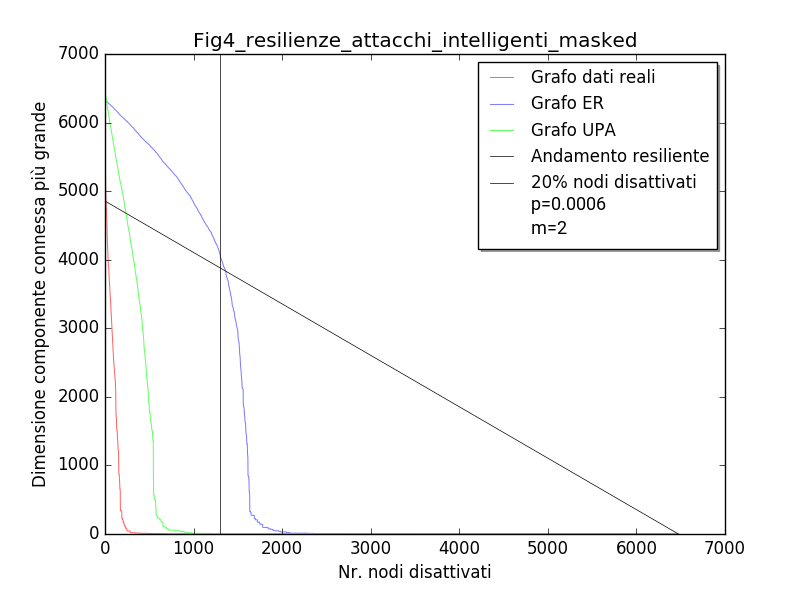
\includegraphics[scale=0.7, \textwidth, left]{Fig4_resilienze_attacchi_intelligenti_masked.png}
\caption{Grafico domanda 4}
\label{fig:graph4}
\end{figure}
\end{center}

Nella figura \ref{fig:graph4} si può notare che solamente il grafo ER è resiliente poichè il punto di intersezione tra la retta verticale indicante il 20\% dei nodi disattivati con la curva del grafo ER (curva blu) è al di sopra della retta che indica se un grafo è resiliente.
Mentre per quanto riguarda gli altri grafi, non sono resiliente poichè dopo l'attacco la dimensione della componente connessa è molto minore al 75\% dei nodi ancora attivi.

\FloatBarrier
\end{document}
